\section{Graphical User Interface}
In this section, we will present and describe the wireframes of the application. These wireframes illustrate the layout and structure of the user interface across different parts of the system, providing a visual representation of how users will interact with the application. Each wireframe focuses on a specific microfrontend or application shell, showcasing its core functionality and design elements.
\subsubsection*{Application Shell}
\begin{figure}[h]
    \centerline{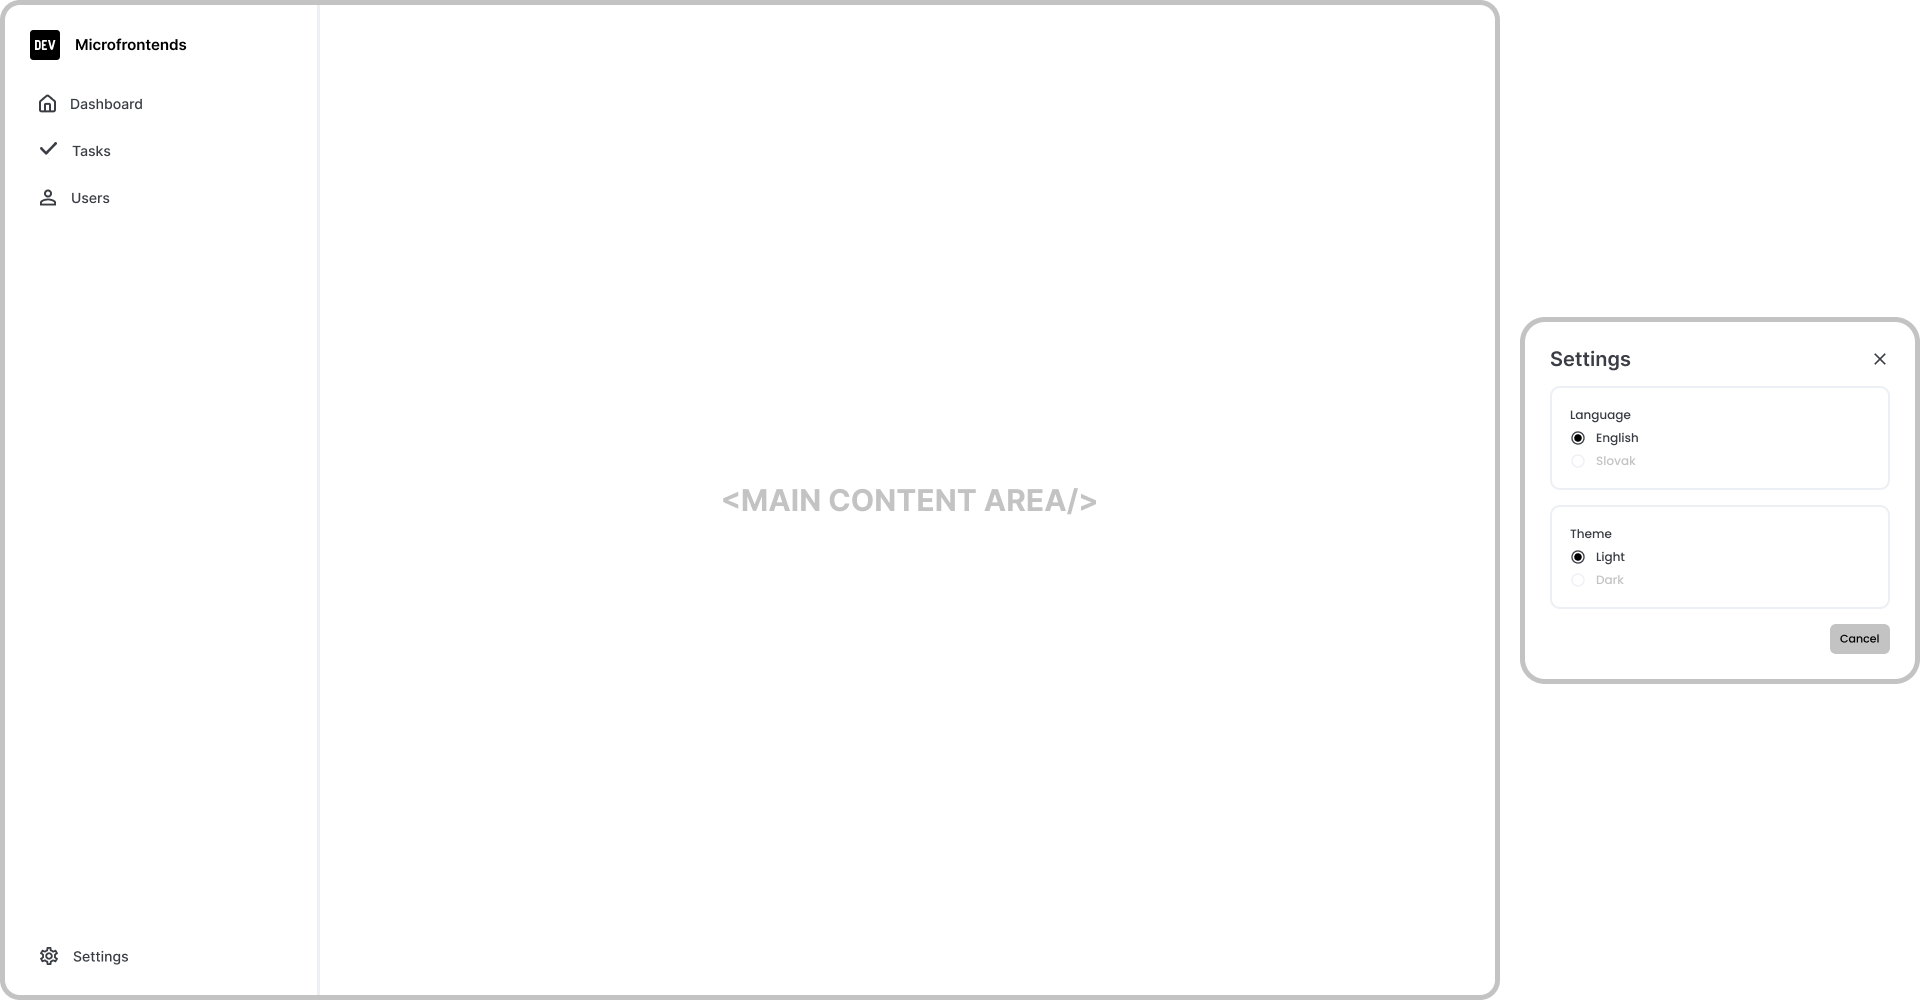
\includegraphics[width=1\textwidth]{images/wireframes/application-shell.png}}
    \caption[Application shell wireframe]{Wireframe of the application shell interface}
    \label{fig:shell-wireframe} 
\end{figure}
As shown in the figure \ref{fig:shell-wireframe}, the application shell consists of a side panel with a logo and navigation links for each microfrontend and a dashboard page. At the bottom of the side panel is a button to open the settings modal, which contains radio buttons for switching the language and application theme. The main content area, next to the side panel, is where all pages will be rendered. This could be either a single microfrontend or the dashboard page.

\subsubsection*{User Microfrontend}
\begin{figure}[h]
\centerline{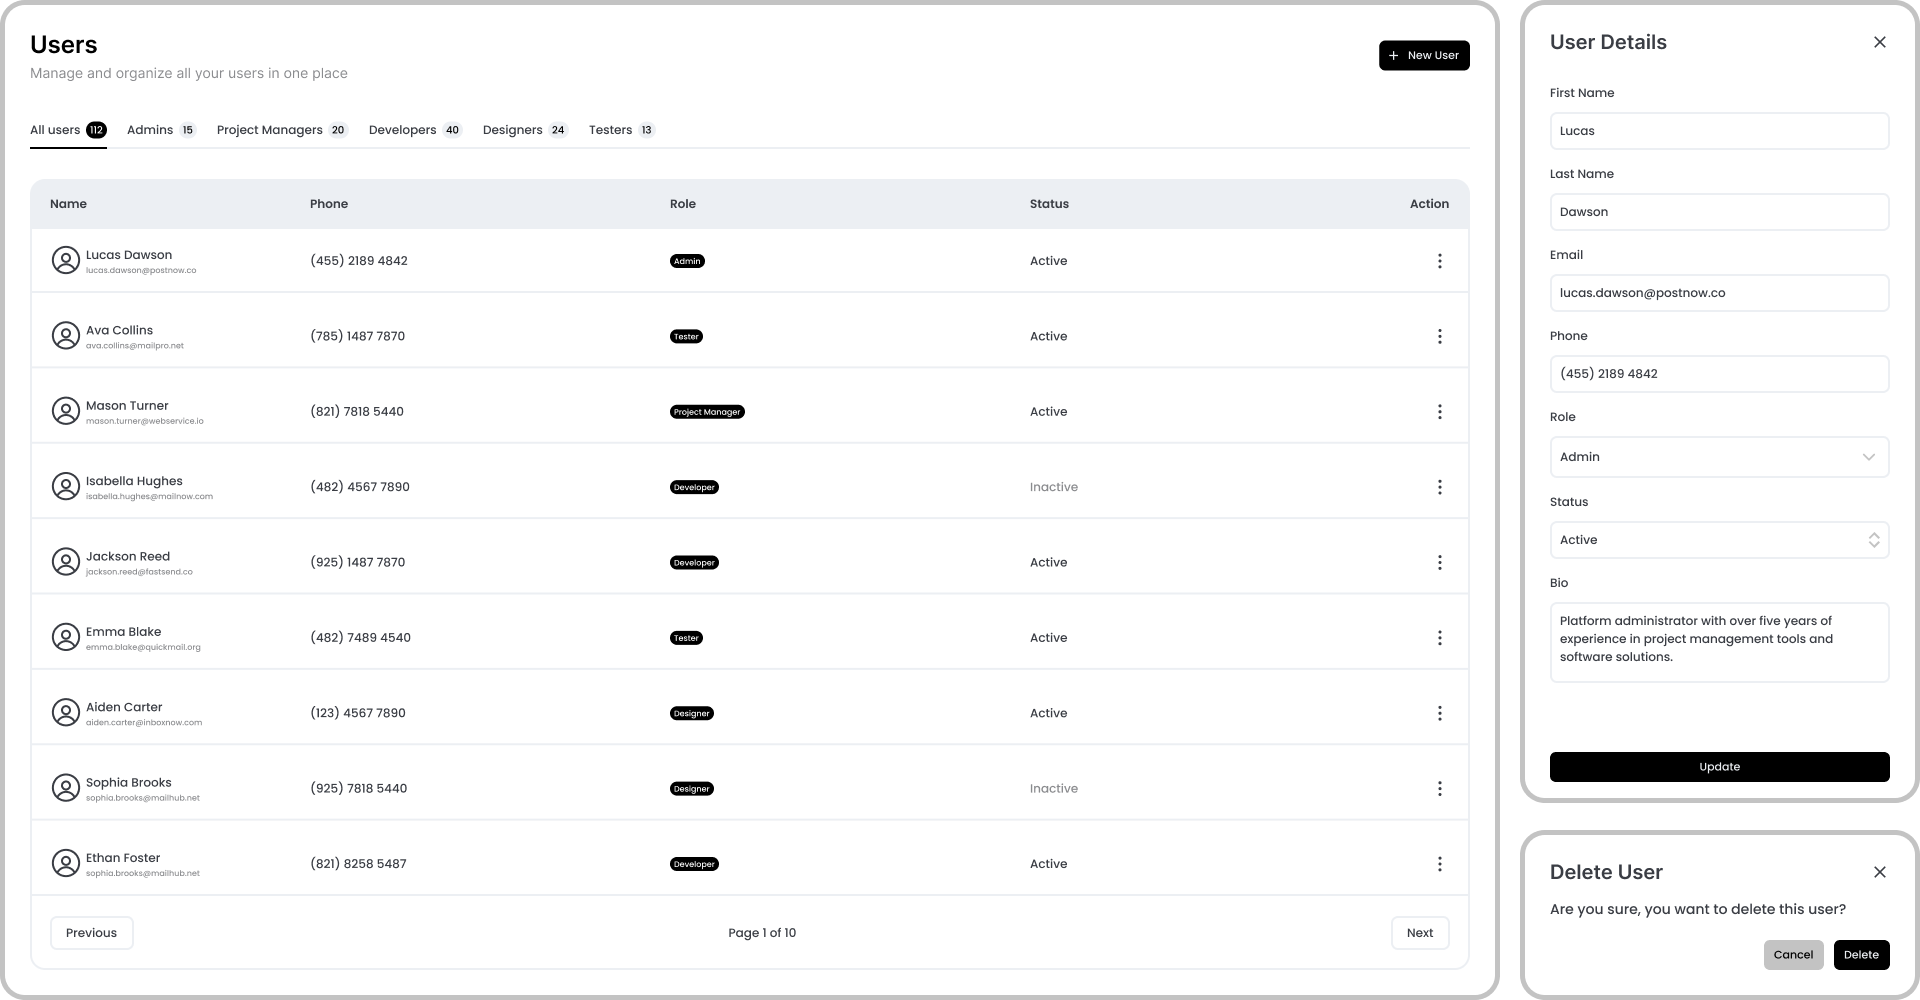
\includegraphics[width=1\textwidth]{images/wireframes/user-microfrontend.png}}
\caption[User microfrontend wireframe]{Wireframe of the user microfrontend interface}
\label{fig:user-wireframe}
\end{figure}
The user microfrontend interface \ref{fig:user-wireframe} consists of a table where each row represents a user, displaying key details such as name, email, phone, role, and status. The last column of the table is dedicated to an action button, which opens a dropdown menu with options to view, edit, or delete a user. Upon selecting any of these actions, a modal window appears, allowing the user to execute the desired operation. Directly above the table is a set of tabs for quick filtering of users based on their roles (e.g., admin, developer, tester, etc.). At the very top, the topbar includes the page title, a brief subtitle, and a button to add a new user. Clicking this button opens a modal for user creation.

\subsubsection*{Task Microfrontend}
\begin{figure}[h]
    \centerline{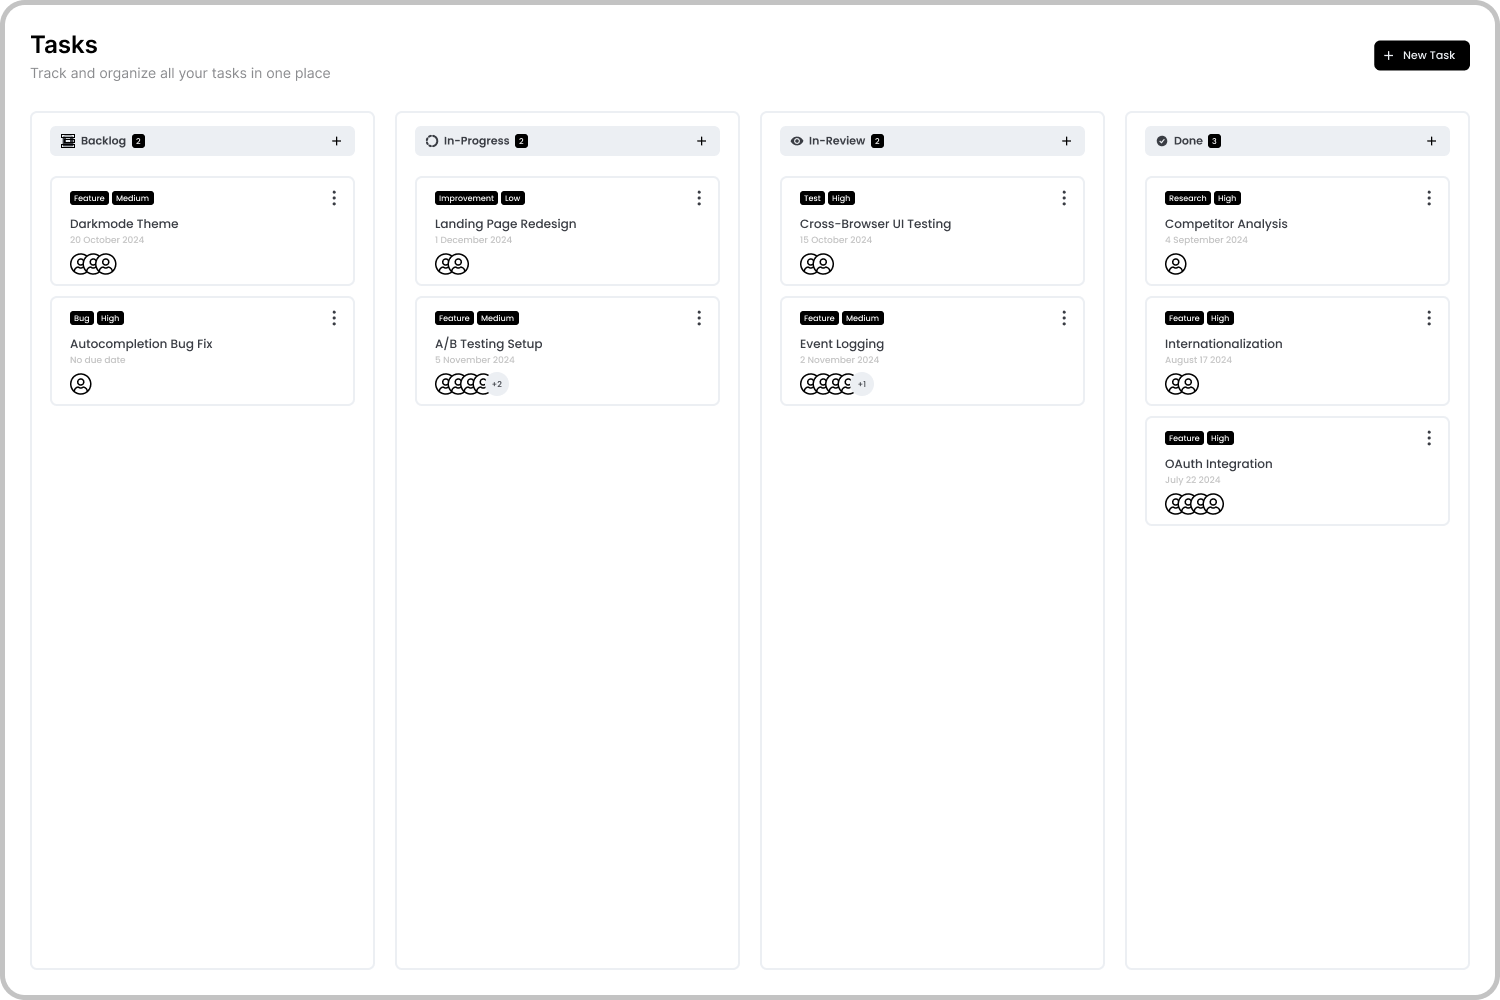
\includegraphics[width=1\textwidth]{images/wireframes/task-microfrontend.png}}
    \caption[Task microfrontend wireframe]{Wireframe of the task microfrontend interface}
    \label{fig:task-wireframe}
\end{figure}
The task microfrontend \ref{fig:task-wireframe} is slightly different from the other sections, as its main component is a kanban board that organizes tasks into various stages, such as ``Backlog'', ``In-Progress'', ``In-Review'' and ``Done''. Each task is represented by a card displaying essential details such as the title, tag, assignees, and more. In the upper-right corner of each task card, there is a three-dot button that opens a dropdown menu with options to view, edit, or delete the task. Upon selecting any of these actions, a modal window appears, allowing the user to execute the desired operation. Each stage on the kanban board includes a button for creating new tasks directly within that stage. At the top of the page is a topbar containing the page title, a brief subtitle, and a button to add a new task. Clicking this button opens a modal designed for task creation.

\subsubsection*{Dashboard}
\begin{figure}[h]
    \centerline{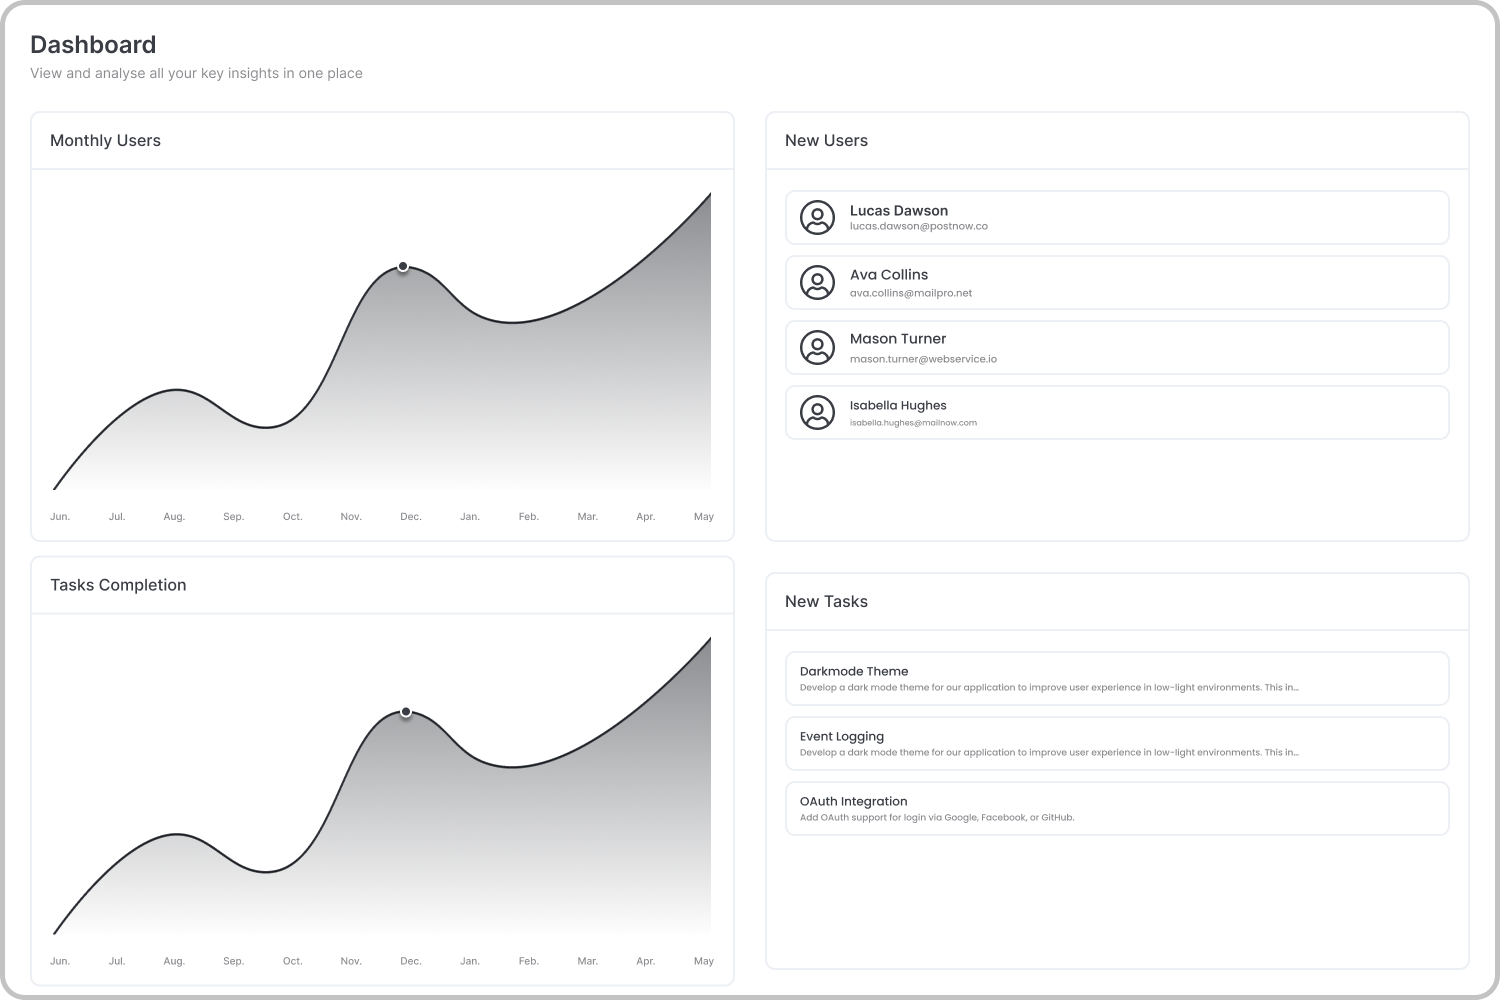
\includegraphics[width=1\textwidth]{images/wireframes/dashboard.png}}
    \caption[Dashboard wireframe]{Wireframe of the dashboard interface}
    \label{fig:dashboard-wireframe}
\end{figure}
The dashboard \ref{fig:dashboard-wireframe} is a combination of the user microfrontend and task microfrontend, both in compact mode, along with application shell elements. At the top of the page is a topbar, which is located in the application shell codebase. Underneath it is the user microfrontend in compact mode, displaying the monthly users graph and the new users widget. At the bottom is the task microfrontend, also in compact mode, displaying the task completion graph and the new tasks widget. These two microfrontends communicate and interact with each other, as already described in the ``System Architecture'' section.